\documentclass{clic_latex_beamer}

%Macros examples
\newcommand{\epfl}{École Polytechnique Fédérale de Lausanne}

\newcommand{\exempleArgs}[2]{
Bonjour #1 et #2 !
}

\usepackage{tikz}
\usepackage{calc}
\newcommand{\exemplePourTous}{
\foreach \x in {1,2,...,3}{$\frac{\sin({\x\pi})}{\x}$+}
$\frac{\sin({4\pi})}{4}$
}

\usepackage{ifthen}
\newcommand{\exempleCondition}[1]{
\ifthenelse{ \equal{#1}{true} }{
  C'est pas faux!
}{
  FAUX!
}
}

%From wikipedia article on macros
\newenvironment{stark}
{ \rule{10ex}{1ex}\hspace{\stretch{1}} }
{ \hspace{\stretch{1}}\rule{10ex}{1ex} }

\begin{document}

\title{Macros et modèles en \LaTeX}
\author{Quentin Mazars-Simon}
\date{\today}
\institute{École Polytechnique Fédérale de Lausanne}
\titlegraphic{\ccbysa}

\frame{\titlepage}


\begin{frame}
\frametitle{Table des matières}
\tableofcontents[]
\end{frame}

%----------------------
%	I - Macros
%----------------------

\section{Macro}
\subsection{À quoi servent les macros ?}
\begin{frame}
\frametitle{À quoi servent les macros ?}
    \begin{itemize}
    \item Définir une macro permet d'automatiser certaines tâches complexes ou répétitives en définissant de nouvelles commandes \LaTeX
    \end{itemize}
 \end{frame}
 
 \subsection{Comment utiliser les macros ?}
 \begin{frame}
\frametitle{Créer une macro}
    \begin{itemize}
    \item Pour définir une macro, on utilise \texttt{\textbackslash newcommand\{\textbackslash nomDeLaMacro\}\{definition\}} 
    \item Par exemple on peut définir la macro suivante: \texttt{\small\textbackslash newcommand\{\textbackslash epfl\}\{École Polytechnique Fédérale de Lausanne\}}\\ et donc en tapant ``\texttt{L'\textbackslash epfl\{\} c'est super !}'' on obtiendra ``L'\epfl{} c'est super!''

    \end{itemize}

 \end{frame}
 
 % ---- Arguments ----
\begin{frame}[fragile]
\frametitle{Utiliser des arguments}
\begin{itemize}
\item Il faut préciser le nombre d'arguments lorsqu'on défini la macro:
\texttt{\textbackslash newcommand\{\textbackslash nomDeLaMacro\}[nombreArgurments]\{\}}
par exemple, \texttt{\textbackslash newcommand\{\textbackslash macroTroisArgs\}[3]\{\}} prendra 3 arguments.
\item Pour accéder aux arguments dans la fonction, on utilise \texttt{\#numéroArgument}, par exemple \texttt{\#2} affichera le 2ème argument.
\item \texttt{\textbackslash exempleArgs\{Robb\}\{Sansa\}} affichera\exempleArgs{Robb}{Sansa}
\begin{lstlisting}
\newcommand{\exempleArgs}[2]{
Bonjour #1 et #2 !
}
\end{lstlisting}
\end{itemize}
\end{frame}
 
 % ---- Conditions ----
\begin{frame}[fragile]
\frametitle{Utiliser des conditions}
\begin{itemize}
\item Il faut importer le package \texttt{ifthen}: \texttt{\textbackslash usepackage\{ifthen\}}
\item Permet d'utiliser les structures de contrôles \texttt{if...then...else...} et \texttt{while...do...} dans les macros
\item Dans cet exemple, \texttt{\textbackslash exempleCondition\{false\}} affichera\exempleCondition{false}
\begin{lstlisting}
\newcommand{\exempleCondition}[1]{
\ifthenelse{ \equal{#1}{true} }{
  C'est pas faux!
}{
  FAUX!
}
}
\end{lstlisting}
\end{itemize}
\end{frame}
 
 % ---- Boucles----
\begin{frame}[fragile]
\frametitle{Utiliser des boucles}
\begin{itemize}
\item Il faut importer le package \texttt{tikz}: \texttt{\textbackslash usepackage\{tikz\}}
\item Permet d'utiliser la structures de contrôles \texttt{foreach...in...} dans les macros
\item Par exemple, la commande  \texttt{\textbackslash exemplePourTous\{\}} affichera\exemplePourTous{}
\begin{lstlisting}
\newcommand{\exemplePourTous}{
\foreach \x in {1,2,...,3}{$\frac{\sin({\x\pi})}{\x}$+}
$\frac{\sin({4\pi})}{4}$
}
\end{lstlisting}
\end{itemize}
\end{frame}
 
 \subsection{Définir de nouveaux environnements}
 \begin{frame}[fragile]
\frametitle{Définir de nouveaux environnements}
\begin{itemize}
\item De manière similaire aux macros, on peut aussi définir de nouveau environnements \texttt{\textbackslash newenvironment{nom}[numArgs]{avant}{après}}
\item \texttt{avant} (resp. \texttt{après}) sera exécuté là où  \texttt{\textbackslash begin\{nom\}} (resp.  \texttt{\textbackslash end\{nom\}}) est écrit.
\item \texttt{\small\textbackslash begin\{stark\}Winter is coming\textbackslash ldots\textbackslash end\{stark\}} nous donne:
\end{itemize}
\begin{stark}Winter is coming\ldots\end{stark}
\begin{lstlisting}
\newenvironment{stark}
{ \rule{10ex}{1ex}\hspace{\stretch{1}} }
{ \hspace{\stretch{1}}\rule{10ex}{1ex} }
\end{lstlisting}
\end{frame}
 
%----------------------------
%	II - Modèles
%----------------------------

% ---- Introduction ----
\section{Modèle}
 \subsection{Qu'est-ce qu'un modèle en \LaTeX}
\begin{frame}
\frametitle{Qu'est-ce qu'un modèle en \LaTeX}
\begin{itemize}
\item Un ensemble de macros regroupées dans un seul fichier.
\item Permet de personnaliser les classes de base pour ses besoins (par exemple, pour son CV).
\item Permet de réutiliser facilement les macros, sans avoir un gros entête au début de chaque fichiers. 
\end{itemize}
 \end{frame}
 
 \begin{frame}
\frametitle{Qu'est-ce qu'un modèle en \LaTeX: exemples}
\centering

\includegraphics[height=\textheight]{illustrations/macros/thesis_exemple.pdf}
 \end{frame}
 
 \begin{frame}
\frametitle{Qu'est-ce qu'un modèle en \LaTeX: exemples}
\centering
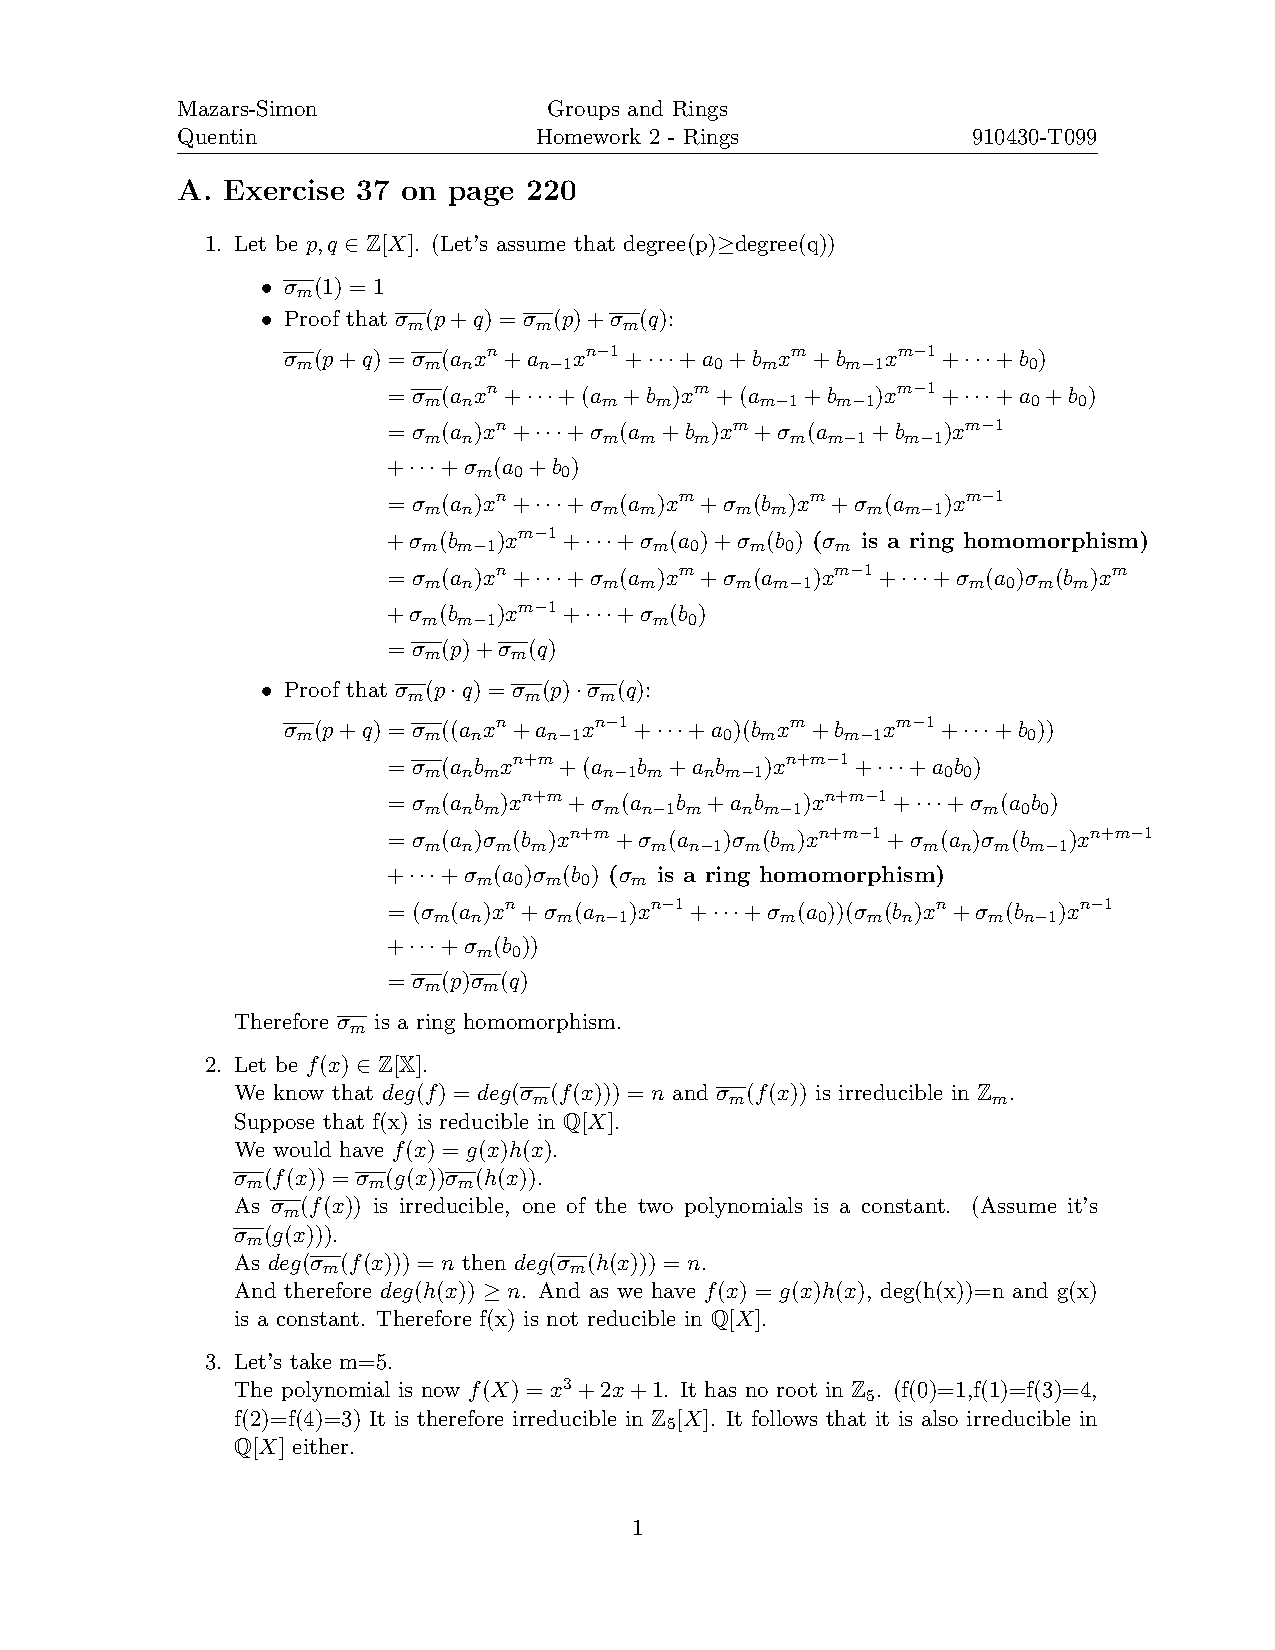
\includegraphics[height=\textheight]{illustrations/macros/serie_exemple.pdf}
 \end{frame}
 
\begin{frame}
\frametitle{Qu'est-ce qu'un modèle en \LaTeX: exemples}
\centering

\includegraphics[height=\textheight]{illustrations/macros/cv_exemple.pdf}
 \end{frame}
 
 % ---- Trouver/Utiliser ----
 \subsection{Où trouver des modèles et comment les utiliser}
 \begin{frame}
\frametitle{Où trouver des modèles et comment les utiliser}
\begin{itemize}
\item Site de l'EPFL {\small\url{http://phd.epfl.ch/thesistemplates}}
\item ShareLatex templates {\small\url{https://www.sharelatex.com/templates/}}
\item WriteLatex templates {\small\url{https://www.writelatex.com/templates/}}
\item Google est votre ami {\small\url{https://www.google.com/search?q=latex+templates}}
\end{itemize}
 \end{frame}
 
\begin{frame}
\frametitle{Où trouver des modèles et comment les utiliser}
\begin{block}{Utiliser un modèle:}
 Utiliser la commande \texttt{\textbackslash documentclass[arguments]\{nom\_du\_modele\}}
\end{block}
Par exemple: \texttt{\textbackslash documentclass\{clic\_latex\_beamer\}}
\begin{alertblock}{Attention}
Par défaut, \LaTeX\ veut que le fichier \texttt{.cls} du modèle soit dans le même dossier que votre \texttt{.tex}
\end{alertblock}
 \end{frame}

% ---- Créer ---- 
\subsection{Créer ses propres modèles}
\begin{frame}[fragile]
\frametitle{Créer ses propres modèles}
 \begin{itemize}
    \item Créer le fichier \texttt{.cls} du modèle (ex: \texttt{clic\_latex.cls})
    \item Déclarer le modèle (versions \LaTeX, nom, description)
\begin{lstlisting}
\NeedsTeXFormat{LaTeX2e}
\ProvidesClass{clic_latex_beamer}[2014/06/03 CLIC's Latex beamer template]
\end{lstlisting}
    \item Importer la classe de base (article, beamer, etc.)
\begin{alertblock}{Attention}
 Il faut utiliser \texttt{\textbackslash LoadClass} au lieu de \texttt{\textbackslash documentclass}
\end{alertblock}
\begin{lstlisting}
\LoadClass[12pt]{beamer}
\end{lstlisting}
      
\end{itemize}
\end{frame}
 
 \begin{frame}[fragile]
\frametitle{Créer ses propres modèles (suite)}
\begin{itemize}
\item Importer les packages nécessaires
\begin{alertblock}{Attention}
 Il faut utiliser \texttt{\textbackslash RequirePackage} au lieu de \texttt{\textbackslash usepackage}
\end{alertblock}
\begin{lstlisting}
\RequirePackage[french]{babel}
\RequirePackage[utf8]{inputenc}
\RequirePackage[T1]{fontenc}
...
\RequirePackage{listings}
\end{lstlisting}
\item Ajouter les diverses customisations, macros, etc.
\begin{lstlisting}
\usetheme{Copenhagen}
\usecolortheme{beaver}
...
\logo{\includegraphics[height=1cm]{clic.png}}
\end{lstlisting}
\end{itemize}
\end{frame}
 
 
%------------------------------------------
%	Questions et Références
%------------------------------------------
 
\begin{frame}
\frametitle{Questions ?}
\begin{center}
\Huge Des questions ?
\end{center}
\end{frame}
 
\begin{frame}
\frametitle{Références}
\begin{itemize}
\item \href{http://en.wikibooks.org/wiki/LaTeX/Macros}{WikiBooks: Latex macros}
\item \href{http://www.sharelatex.com/learn/Defining_your_own_commands}{ShareLatex: Defining your own commands}
\item \href{https://www.sharelatex.com/blog/2011/03/27/how-to-write-a-latex-class-file-and-design-your-own-cv.html}{Sharelatex: How to write a LaTeX class file and design your own CV}
\end{itemize}
\end{frame}


\end{document}
